The goal of this chapter is to evaluate the proposed \textit{Invox} system and analyze its performance across multiple extraction strategies using the \textbf{MUC-4 benchmark dataset}. The evaluation aims to measure how effectively the system transforms unstructured, noisy text into structured templates under real-world conditions. To this end, the assessment focuses on the dimensions of \textbf{accuracy}, \textbf{consistency}, \textbf{latency}, \textbf{cost}, and \textbf{modularity}, in direct correspondence with the requirements defined in Chapter~\ref{chap:analysis}.

Unlike traditional information extraction evaluations that rely on strict lexical overlap, the MUC-4 dataset poses a distinctive challenge: both the gold standard and system predictions may include \textit{multiple valid fillers} per slot, expressed through paraphrases or partial phrases. A purely string-based comparison would therefore underestimate performance. To account for this, all evaluations employ an \textbf{embedding-based semantic framework} in which cosine similarity between gold and predicted values captures conceptual correctness rather than surface form matching. This provides a fairer, more robust measure of information extraction quality.

The chapter proceeds as follows. Section~\ref{sec:eval-dataset} introduces the MUC-4 dataset and the preprocessing pipeline applied prior to evaluation. Section~\ref{sec:eval-metrics} defines the semantic similarity metrics and auxiliary measures such as latency and cost. Section~\ref{sec:eval-setup} describes the experimental setup and the evaluated strategies. Sections~\ref{sec:eval-langextract}--\ref{sec:eval-comparative} present quantitative and qualitative results, followed by a summary that relates the findings to the original design requirements.

\section{Datasets}
\label{sec:eval-dataset}

The evaluation datasets are curated sets of JavaScript and TypeScript vulnerability test cases maintained alongside the Code Guardian prototype in \texttt{code-guardian/evaluation/datasets/}. Each test case consists of (i) a short code snippet, (ii) a list of expected vulnerabilities with CWE identifiers and severities, and (iii) an expected remediation description. Two datasets are provided:
\begin{itemize}
  \item \textbf{Core dataset:} \texttt{vulnerability-test-cases.json} contains representative examples for common vulnerability classes (e.g., SQL injection, XSS, command injection, path traversal) as well as a small number of secure examples to measure false positives.
  \item \textbf{Advanced dataset:} \texttt{advanced-test-cases.json} contains additional vulnerability types and more nuanced patterns (e.g., insecure CORS configuration, timing attacks, mass assignment).
\end{itemize}

In the current prototype version, the core dataset contains \textbf{20} test cases (\textbf{18} vulnerable and \textbf{2} secure), and the advanced dataset contains \textbf{28} test cases (\textbf{25} vulnerable and \textbf{3} secure). Expected findings in both datasets are annotated with CWE identifiers to support aggregation by vulnerability class.

\paragraph{Which dataset is scored by default.}
The repository-contained evaluation harness used in this thesis (\texttt{code-guardian/evaluation/evaluate-models.js}) loads and scores the \emph{core} dataset by default. The advanced dataset is included to broaden coverage and can be evaluated by extending the harness to load an additional JSON file or to run two passes (core vs.\ advanced). Unless stated otherwise, quantitative results in Chapter~\ref{chap:evaluation} refer to the core dataset.

Vulnerability classes are aligned with the Common Weakness Enumeration taxonomy \cite{mitreCWE}, and severities are recorded as coarse labels to support prioritization and reporting. Where applicable, severity can be related back to standardized scoring systems such as CVSS and public vulnerability databases such as CVE/NVD \cite{firstCvss31,mitreCVE,nistNVD}.

This dataset targets requirement R2 (context-aware vulnerability reasoning) by including vulnerability instances that cannot be resolved purely by superficial keyword matching (e.g., sink usage that requires reasoning about tainted input). It also supports R1 by enabling reproducible comparisons across repeated runs and across different local models.

\subsection*{Dataset Schema}

Each record follows a uniform schema:
\begin{itemize}
  \item \texttt{id}: unique identifier
  \item \texttt{name}: descriptive test name
  \item \texttt{code}: code snippet under test
  \item \texttt{expectedVulnerabilities}: list of expected findings (type, CWE, severity, description)
  \item \texttt{expectedFix}: short remediation guidance (optional)
\end{itemize}

The dataset is intentionally small and human-auditable to facilitate iteration on prompts, retrieval, and output validation. Limitations of synthetic snippets and representativeness are discussed in Section~\ref{sec:eval-summary}.

\paragraph{Toward larger benchmarks.}
While this thesis focuses on a curated, auditable suite to support rapid iteration, standard benchmark suites such as the OWASP Benchmark and NIST Juliet can be used to broaden coverage and stress-test generalization in future work \cite{owaspBenchmark,nistJuliet}. In addition, secure coding checklists and verification frameworks such as OWASP ASVS can guide the selection of security requirements and test categories when scaling the evaluation \cite{owaspASVS}.

\section{Evaluation Metrics}
\label{sec:eval-metrics}

We evaluate Code Guardian along complementary axes aligned with Chapter~\ref{chap:analysis}: detection quality (R1--R2), explainability/structure (R3), and responsiveness (R6).

\subsection*{Detection Quality}

Given an expected set of vulnerability types per test case and a detected set of vulnerability types returned by the model, we compute:
\begin{itemize}
  \item \textbf{Precision:} $\mathrm{TP}/(\mathrm{TP}+\mathrm{FP})$
  \item \textbf{Recall:} $\mathrm{TP}/(\mathrm{TP}+\mathrm{FN})$
  \item \textbf{F1 score:} harmonic mean of precision and recall
  \item \textbf{False positive rate (FPR):} $\mathrm{FP}/(\mathrm{FP}+\mathrm{TN})$ on secure examples
  \item \textbf{Accuracy:} $(\mathrm{TP}+\mathrm{TN})/N$
\end{itemize}

Matching is performed at the vulnerability-type level. To account for naming variation (e.g., ``Cross-Site Scripting'' vs.\ ``XSS''), the evaluation script applies case-insensitive substring matching between expected and detected type strings.

\paragraph{Secure examples.}
The datasets include a small number of intentionally secure snippets (core: 2; advanced: 3). These examples are used to estimate the false positive rate and to sanity-check whether a model tends to over-warn under strict JSON output constraints.

\subsection*{Structured Output Robustness}

Because Code Guardian integrates findings into IDE diagnostics, structured output is essential. We therefore report:
\begin{itemize}
  \item \textbf{JSON parse success rate:} percentage of responses that parse into a JSON array of issues.
\end{itemize}

\paragraph{How parse failures are treated.}
In the evaluation harness, responses that do not parse as a JSON array are counted as parse failures and are scored as producing an empty set of issues. For vulnerable test cases, this manifests as false negatives (missed findings); for secure test cases, it can appear as a true negative but still indicates that the system is not usable for IDE automation. Reporting parse success rate separately is therefore important to avoid over-interpreting accuracy numbers when a model frequently produces malformed output.

\subsection*{Responsiveness}

We measure:
\begin{itemize}
  \item \textbf{Response time:} wall-clock time per analysis call (milliseconds), summarized by mean and median.
\end{itemize}

Latency is interpreted in the context of IDE workflows: function-level analysis has tighter budgets than file-level or workspace scans.

\paragraph{Limits of the scoring setup.}
The current quantitative scoring focuses on vulnerability-type detection rather than exact localization quality. This is a deliberate choice aligned with the harness design (type strings and severities are available for scoring), but it means that line-range accuracy and patch minimality are evaluated qualitatively rather than through automated metrics.

\section{Experimental Setup}
\label{sec:eval-setup}

All experiments are executed locally using the Code Guardian evaluation harness in \path{code-guardian/evaluation/evaluate-models.js}. The harness iterates over the curated dataset described in Section~\ref{sec:eval-dataset} and invokes Ollama with a strict JSON-only system prompt. Model decoding is configured for low randomness (\texttt{temperature=0.1}) to improve determinism and parsing stability.

\subsection*{Response Schema for Scoring}

For evaluation purposes, the harness requests a richer structured output than the minimal in-editor diagnostics flow. In particular, each finding includes a vulnerability \texttt{type} string and a coarse \texttt{severity} level in addition to location and an optional fix. This enables type-level scoring (precision/recall) and per-category analysis. In the extension UI, vulnerability categories may appear within the message text and are used for downstream aggregation (e.g., in the workspace dashboard); a future refinement is to surface \texttt{type} and \texttt{severity} as first-class fields in diagnostics.

\subsection*{Compared Configurations}

Two configurations are evaluated quantitatively:
\begin{itemize}
  \item \textbf{LLM-only:} JSON-only analyzer without retrieval context.
  \item \textbf{LLM+RAG:} retrieval-augmented prompting with static security snippets (\texttt{k=5}).
\end{itemize}

Where relevant, results can also be stratified by model size or model family to study the trade-off between accuracy and latency.

\subsection*{Models and Hardware}

The reported run used two local Ollama models: \texttt{gemma3:1b} and \texttt{qwen3-coder}. In runtime metadata, the second model resolves to the latest local tag. The execution environment was macOS (Darwin 25.3.0, arm64) on Apple M4 Max (16 CPU cores, 64\,GB RAM), Node.js v20.19.5, and Ollama 0.17.0.

\subsection*{Runtime Parameters}

The evaluation harness enforces a per-request timeout (\texttt{timeoutMs=30000}) and limits generation length (\texttt{num\_predict=1000}). A request delay of \texttt{500\,ms} is inserted between calls to reduce burstiness on developer hardware. Runs were executed sequentially with no warm-up and no retries.

\subsection*{Reproducibility Snapshot}

\begin{table}[H]
  \centering
  \caption{Run configuration used for reported results.}
  \label{tab:eval-reproducibility}
  \small
  \begin{tabular}{p{0.33\textwidth}p{0.6\textwidth}}
    \toprule
    Item & Value \\
    \midrule
    Dataset file & \texttt{vulnerability-test-cases.json} (33 cases: 18 vulnerable, 15 secure) \\
    Runs per sample & 3 \\
    Prompt modes & LLM-only, LLM+RAG \\
    RAG settings & static security snippets, \texttt{k=5} \\
    Generation settings & \texttt{temperature=0.1}, \texttt{num\_predict=1000} \\
    Request controls & \texttt{timeoutMs=30000}, \texttt{requestDelayMs=500} \\
    Execution mode & sequential, no warm-up, no retries \\
    Models requested & \texttt{gemma3:1b}, \texttt{qwen3-coder} \\
    Model resolution & \texttt{qwen3-coder} $\rightarrow$ \texttt{qwen3-coder:latest} \\
    Software & Ollama 0.17.0, Node.js v20.19.5 \\
    Hardware/OS & Apple M4 Max (16 CPU cores, 64 GB RAM), macOS Darwin 25.3.0 (arm64) \\
    \bottomrule
  \end{tabular}
\end{table}

\subsection*{Artifact Provenance}

To make the evaluation independently auditable, Table~\ref{tab:eval-artifact-manifest} records the provenance fingerprint for the reported run.

\begin{table}[H]
  \centering
  \caption{Artifact provenance manifest for this thesis run.}
  \label{tab:eval-artifact-manifest}
  \footnotesize
  \begin{tabularx}{\textwidth}{p{0.34\textwidth}X}
    \toprule
    Field & Value \\
    \midrule
    Thesis repository commit & \texttt{82d24c4fdb13} \\
    Run window (UTC) & 2026-02-24 20:33:15 to 2026-02-24 20:41:33 \\
    Total runtime & 497\,841 ms \\
    Execution policy & sequential order, no retries, no warm-up \\
    Dataset path & \path{code-guardian/evaluation/datasets/vulnerability-test-cases.json} \\
    Invocation command & \texttt{node evaluation/evaluate-models.js} \\
    Model fingerprint (gemma3:1b) & digest prefix \texttt{8648f39daa8f} \\
    Model fingerprint (qwen3-coder:latest) & digest prefix \texttt{06c1097efce0} \\
    \bottomrule
  \end{tabularx}
\end{table}

For archival reproducibility, the recommended artifact bundle includes: (i) raw JSON output from the harness, (ii) the exact run configuration object, (iii) model digests, and (iv) generated summary tables. These artifacts should be stored as supplementary material together with the thesis PDF.

\subsection*{Uncertainty Estimation}

Each sample is evaluated three times. In this thesis, uncertainty is summarized with 95\% Wilson confidence intervals for:
\begin{itemize}
  \item \textbf{Recall} (denominator: vulnerable evaluations, $n=54$), and
  \item \textbf{Parse success} (denominator: total requests, $n=99$).
\end{itemize}
We do not report formal confidence intervals for precision and FPR because the current harness counts issue-level false positives, which makes those denominators less directly comparable across configurations.

\paragraph{Response parsing.}
The harness strips Markdown code fences if present and then attempts to parse the remaining content as JSON. Responses that fail to parse are counted toward the parse failure rate and are scored as producing no issues, which impacts recall on vulnerable samples.

\subsection*{Running the Evaluation}

The evaluation can be reproduced by running:
\begin{lstlisting}[language=Java, caption={Running the Code Guardian evaluation harness}, label={lst:eval-run}]
cd code-guardian
node evaluation/evaluate-models.js
\end{lstlisting}

The script produces per-model metrics and can be extended to emit JSON/Markdown reports under \path{code-guardian/evaluation/logs/} for inclusion in the thesis appendix.

The reported results in this thesis were produced with \texttt{runsPerSample=3} for both prompt modes.

\section{Results – LangExtract Baseline (S5)}
\label{sec:eval-langextract}

\textbf{LangExtract} is an open-source, LLM-powered Python library for schema-constrained extraction. In this work it is used as an external baseline rather than a core component of the proposed system: it provides a deterministic orchestration wrapper around model calls (strict JSON schema enforcement and span grounding), but is not integrated into the multi-agent architecture.

On the MUC-4 subset ($N{=}100$ documents), LangExtract achieves an overall balanced score (OBS) of $0.684$ and a format-driven accuracy (FDA) of $0.756$, with a relatively low hallucination rate (HR) of $0.088$ and a high rate of fully correct fields (RFA $=0.796$) (see Table~\ref{tab:langextract-headline} in Appendix~\ref{appendix:detailed-results}). This pattern indicates a conservative filler: when the system commits to a value it is usually accurate, but it frequently abstains. The non-empty specific metrics reflect this behaviour: the non-empty $F_1$ score remains modest ($0.406$), and the non-empty exact accuracy (EAI) of $0.182$ shows that much of the performance comes from correctly leaving fields empty when the gold label is empty.

Field-wise analysis (Table~\ref{tab:langextract-perfield}) reveals a skew towards easier categorical slots such as \texttt{incidentType}, \texttt{weapon}, and \texttt{incidentStage}, which achieve comparatively high scores, whereas more complex or ambiguous fields such as \texttt{target}, \texttt{incidentLocation}, and especially \texttt{perpetratorOrganization} perform noticeably worse under gold-nonempty evaluation. The \texttt{incidentDate} field is particularly under-filled: in cases where the gold label is nonempty, the model often abstains, contributing to the higher miss rate (MR $=0.369$).

The embedding-based metrics in Table~\ref{tab:langextract-embed-overall} and Table~\ref{tab:langextract-embed-perfield} confirm that LangExtract produces stylistically consistent outputs with reasonable semantic coverage: soft coverage and specificity are balanced, and the symmetric Chamfer scores are stable across text and list fields. Consistency metrics (schema format vs.\ style, see Appendix~\ref{appendix:detailed-implementation}) show perfect schema adherence ($\mathrm{FPR}_{\text{overall}}=1.000$) and a style consistency score of $\mathrm{SC}_{\text{macro}}=0.709$, which is comparable to the best multi-agent strategies.

In terms of runtime, LangExtract exhibits moderate latency, with a median of approximately $21$\,s per document and a long tail extending to around $110$\,s (Table~\ref{tab:langextract-latency}). This makes it practical as a batch or asynchronous baseline, but less attractive as an interactive component. Overall, S5 serves as a useful external point of comparison: it demonstrates that a mature off-the-shelf extractor can reach solid accuracy under conservative filling, but it does not outperform the best multi-agent strategies in the non-empty and robustness-oriented metrics that are central to this thesis.

\section{Results: LLM-Only Configuration}
\label{sec:eval-llm-only}

This section reports results for Code Guardian when operating without retrieval augmentation. The goal is to establish a baseline for detection quality and latency when the model receives only the analyzed code and strict JSON-output constraints.

\subsection*{Detection Quality}

Table~\ref{tab:eval-llm-only} summarizes precision, recall, and F1 score on the curated dataset. These values should be reported per model, as different local models can show distinct precision/recall trade-offs.

\begin{table}[H]
  \centering
  \caption{LLM-only evaluation metrics on the curated dataset (fill with measured values).}
  \label{tab:eval-llm-only}
  \begin{tabular}{lccccc}
    \toprule
    Model & Precision (\%) & Recall (\%) & F1 (\%) & FPR (\%) & Parse rate (\%) \\
    \midrule
    \texttt{<model-1>} & -- & -- & -- & -- & -- \\
    \texttt{<model-2>} & -- & -- & -- & -- & -- \\
    \bottomrule
  \end{tabular}
\end{table}

\subsection*{Latency}

For interactive usage, response time is critical. Table~\ref{tab:eval-llm-only-latency} reports median and mean latency per analysis call for each model under the evaluation harness.

\begin{table}[H]
  \centering
  \caption{LLM-only latency metrics (fill with measured values).}
  \label{tab:eval-llm-only-latency}
  \begin{tabular}{lcc}
    \toprule
    Model & Median (ms) & Mean (ms) \\
    \midrule
    \texttt{<model-1>} & -- & -- \\
    \texttt{<model-2>} & -- & -- \\
    \bottomrule
  \end{tabular}
\end{table}

\subsection*{Discussion}

The LLM-only configuration is typically the lowest-latency option and is therefore suitable for real-time feedback in the editor. However, without grounding, it can be more sensitive to hallucinations and may produce less consistent classifications for borderline patterns. The next section evaluates whether retrieval augmentation improves grounding and reduces false positives.

\section{Results: LLM+RAG Configuration}
\label{sec:eval-rag}

This section reports Code Guardian with retrieval augmentation enabled. In this configuration, the prompt is enriched with locally retrieved security knowledge (CWE/OWASP/CVE-derived summaries and mitigation guidance) to ground the model’s output.

\subsection*{Detection Quality}

Table~\ref{tab:eval-rag} summarizes detection metrics for the RAG-enhanced configuration. Comparing Table~\ref{tab:eval-rag} against Table~\ref{tab:eval-llm-only} isolates the empirical impact of retrieval augmentation on precision/recall trade-offs.

\begin{table}[H]
  \centering
  \caption{LLM+RAG evaluation metrics on the curated dataset.}
  \label{tab:eval-rag}
  \small
  \begin{tabular}{lccccc}
    \toprule
    Model & Precision (\%) & Recall (\%) & F1 (\%) & FPR (\%) & Parse rate (\%) \\
    \midrule
    \texttt{gemma3:1b} & 0.00 & 0.00 & 0.00 & 0.00 & 100.00 \\
    \texttt{qwen3-coder} & 27.27 & 55.56 & 36.59 & 100.00 & 100.00 \\
    \bottomrule
  \end{tabular}
\end{table}

\subsection*{Latency Overhead}

Retrieval introduces overhead from embedding, vector search, and prompt expansion. Table~\ref{tab:eval-rag-latency} reports the latency impact of enabling RAG under the same evaluation harness.

\begin{table}[H]
  \centering
  \caption{LLM+RAG latency metrics.}
  \label{tab:eval-rag-latency}
  \small
  \begin{tabular}{lcc}
    \toprule
    Model & Median (ms) & Mean (ms) \\
    \midrule
    \texttt{gemma3:1b} & 182 & 185 \\
    \texttt{qwen3-coder} & 1060 & 1140 \\
    \bottomrule
  \end{tabular}
\end{table}

\subsection*{Discussion}

RAG effects are model-dependent in this run. For \texttt{qwen3-coder}, RAG improved precision, recall, and F1 while also reducing latency compared to its LLM-only configuration. For \texttt{gemma3:1b}, RAG collapsed recall to zero and produced no true positives. This indicates that retrieval augmentation improved performance only when the base model could effectively incorporate retrieved context.

\section{Model Comparison and Category Breakdown}
\label{sec:eval-models}

Code Guardian supports multiple local models through Ollama. In practice, model choice affects not only detection quality but also structured-output robustness and latency. This section summarizes the measured ablation results and category-level behavior observed in the run logs.

\subsection*{Ablation Comparison}

Table~\ref{tab:eval-ablation-summary} compares all measured model/prompt-mode combinations.

\begin{table}[H]
  \centering
  \caption{Ablation summary across model and prompt mode.}
  \label{tab:eval-ablation-summary}
  \resizebox{\textwidth}{!}{%
  \begin{tabular}{lcccccc}
      \toprule
      Configuration & Precision (\%) & Recall (\%) & F1 (\%) & FPR (\%) & Parse (\%) & Median (ms) \\
      \midrule
      \texttt{qwen3:8b} (LLM+RAG) & 54.29 & 35.19 & 42.70 & 27.12 & 84.85 & 7809 \\
      \texttt{qwen3:8b} (LLM-only) & 38.30 & 33.33 & 35.64 & 39.73 & 77.78 & 8774 \\
      \texttt{gemma3:4b} (LLM+RAG) & 24.24 & 44.44 & 31.37 & 100.00 & 100.00 & 1335 \\
      \texttt{gemma3:4b} (LLM-only) & 23.96 & 42.59 & 30.67 & 100.00 & 96.97 & 1415 \\
      \texttt{gemma3:1b} (LLM-only) & 100.00 & 5.56 & 10.53 & 0.00 & 100.00 & 178 \\
      \texttt{CodeLlama:latest} (LLM-only) & 40.00 & 3.70 & 6.78 & 6.25 & 5.05 & 3987 \\
      \texttt{gemma3:1b} (LLM+RAG) & 0.00 & 0.00 & 0.00 & 0.00 & 100.00 & 180 \\
      \texttt{qwen3:4b} (LLM-only) & 0.00 & 0.00 & 0.00 & 0.00 & 1.01 & 9549 \\
      \texttt{qwen3:4b} (LLM+RAG) & 0.00 & 0.00 & 0.00 & 0.00 & 4.04 & 9852 \\
      \texttt{CodeLlama:latest} (LLM+RAG) & 0.00 & 0.00 & 0.00 & 10.00 & 1.01 & 5478 \\
      \bottomrule
    \end{tabular}%
  }
\end{table}

\subsection*{Per-Category Observations}

Based on detailed run logs, injection-style cases (SQL injection and XSS) were consistently detected by \texttt{qwen3:8b} in the best-performing configuration. At the same time, representative misses remained (e.g., NoSQL injection), and secure samples still produced false alarms in several configurations. The most extreme alert-noise behavior appears in \texttt{gemma3:4b}, where secure evaluations were flagged in every run (FPR 100\% in both modes).

\subsection*{Interpretation}

These results motivate two practical follow-ups: stronger output-contract enforcement for models with low parse reliability, and stricter abstention behavior on secure samples for high-noise configurations. They also support differentiated defaults: a fast conservative model for inline checks and a higher-accuracy model for audit mode when higher latency is acceptable.

\section{Results – Strategy S4: Multi-LLM Per-Field}
\label{sec:eval-s4}

The \textbf{S4: Multi-LLM Per-Field} strategy applies consensus at the slot level: each field is extracted by multiple models and consolidated via a field-aware verifier. We evaluate three variants: \textbf{S4.0} without few-shot prompting on the original MUC-4 dataset, \textbf{S4.1} with few-shot prompting on the original dataset, and \textbf{S4.2} with few-shot prompting on a speech-style variant.

Figure~\ref{fig:s4-variants-bar} shows that per-field consensus behaves differently from the other strategies: it produces strong nonempty-field performance (high NES) but tends to overfill slots, as reflected in the negative EAI values and elevated hallucination rates. This indicates that the model ensemble is biased toward producing a value rather than abstaining. Few-shot prompting moderates this behaviour slightly by reducing hallucinations and improving overall accuracy, though the conservative–vs.–aggressive fill trade-off persists. The speech-style variant remains close to the clean-text version, showing that slot-wise consensus dampens some noise effects but does not fully counteract the tendency to oversupply values.

Per-field consensus boosts \texttt{incidentLocation}; \texttt{perpetratorIndividual} remains hardest; \texttt{weapon} is lower than in S1 and S3.

Figure ~\ref{fig:s4-perfield-plot} illustrates the asymmetric effects of per-field voting on different slots. \texttt{incidentLocation} benefits most, reaching an average score of $0.641$ in S4.1 and surpassing the corresponding values in the single-pass and full-document consensus strategies, which suggests that slot-specific prompts plus ensemble agreement help to stabilise location predictions. \texttt{incidentStage} also performs strongly ($0.720$), consistent with its comparatively structured label space. In contrast, \texttt{incidentType} and especially \texttt{incidentDate} underperform relative to other strategies (down to $0.370$ for dates), which indicates that aggressive filling at the field level can lead to more spurious or partially incorrect outputs when the signal is weak. \texttt{weapon} achieves $0.692$, clearly lower than in S1 and S3, suggesting that per-field voting may over-accept marginal mentions and noise in this slot. \texttt{perpetratorIndividual} remains one of the hardest fields despite the richer consensus mechanism, reflecting the persistent difficulty of sparse, ambiguous references to individual actors.

\begin{figure}[H]
\centering
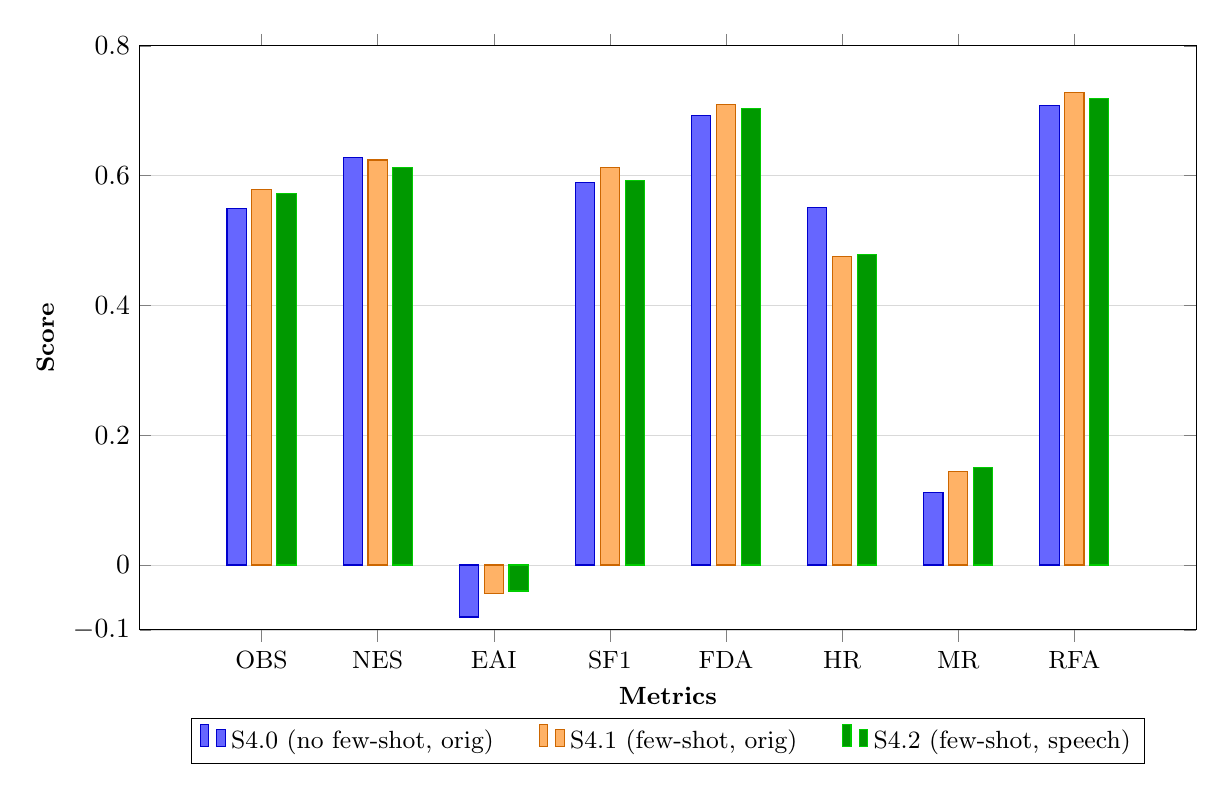
\begin{tikzpicture}
  \begin{axis}[
    width=15cm,
    height=9cm,
    ybar,
    bar width=7pt,
    ylabel={Score},
    ylabel style={font=\small\bfseries},
    xlabel={Metrics},
    xlabel style={font=\small\bfseries},
    symbolic x coords={OBS, NES, EAI, SF1, FDA, HR, MR, RFA},
    xtick=data,
    xticklabel style={font=\small},
    ymin=-0.1,
    ymax=0.8,
    ytick={-0.1, 0, 0.2, 0.4, 0.6, 0.8},
    ymajorgrids=true,
    grid style={line width=0.3pt, draw=gray!30},
    legend style={
      at={(0.5,-0.15)},
      anchor=north,
      legend columns=3,
      font=\small,
      /tikz/every even column/.append style={column sep=0.5cm}
    },
    enlarge x limits=0.15,
  ]
  
  % S4.0 (no few-shot, orig) - Blue
  \addplot[fill=blue!60, draw=blue!80!black] coordinates {
    (OBS, 0.549)
    (NES, 0.628)
    (EAI, -0.080)
    (SF1, 0.589)
    (FDA, 0.693)
    (HR, 0.551)
    (MR, 0.112)
    (RFA, 0.708)
  };
  \addlegendentry{S4.0 (no few-shot, orig)}
  
  % S4.1 (few-shot, orig) - Orange
  \addplot[fill=orange!60, draw=orange!80!black] coordinates {
    (OBS, 0.579)
    (NES, 0.624)
    (EAI, -0.044)
    (SF1, 0.613)
    (FDA, 0.709)
    (HR, 0.476)
    (MR, 0.144)
    (RFA, 0.728)
  };
  \addlegendentry{S4.1 (few-shot, orig)}
  
  % S4.2 (few-shot, speech) - Green
  \addplot[fill=green!60!black, draw=green!80!black] coordinates {
    (OBS, 0.572)
    (NES, 0.612)
    (EAI, -0.040)
    (SF1, 0.592)
    (FDA, 0.704)
    (HR, 0.479)
    (MR, 0.150)
    (RFA, 0.719)
  };
  \addlegendentry{S4.2 (few-shot, speech)}
  
  \end{axis}
\end{tikzpicture}
\caption{Headline metrics for S4 variants on MUC-4 ($N{=}100$). Few-shot prompting (S4.1) improves most accuracy-oriented metrics (OBS, SF1, FDA, RFA) but still produces negative EAI values, indicating disagreement across models at the slot level. The speech-style variant (S4.2) performs similarly to S4.1, suggesting that per-field consensus mitigates some ASR-related noise. Overall, S4 offers strong schema adherence but also highlights how per-field aggregation can amplify model inconsistencies.}
\label{fig:s4-variants-bar}
\end{figure}



\begin{figure}[H]
\centering
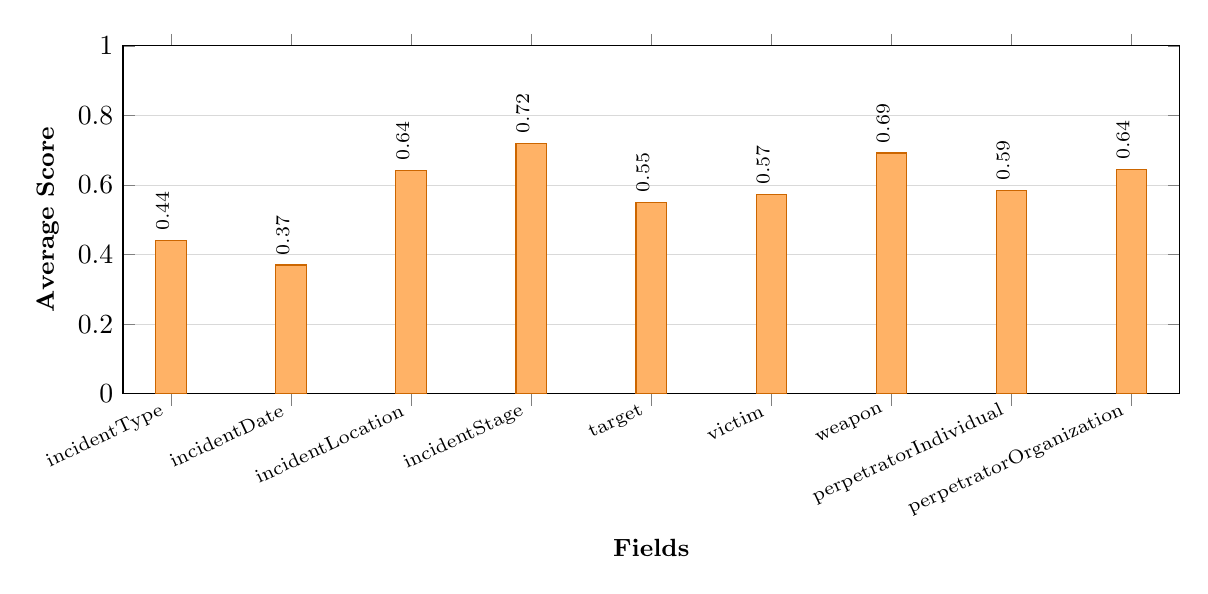
\begin{tikzpicture}
  \begin{axis}[
    width=15cm,
    height=6cm,
    ybar,
    bar width=11pt,
    ylabel={Average Score},
    ylabel style={font=\small\bfseries},
    xlabel={Fields},
    xlabel style={font=\small\bfseries},
    symbolic x coords={
      incidentType,
      incidentDate,
      incidentLocation,
      incidentStage,
      target,
      victim,
      weapon,
      perpetratorIndividual,
      perpetratorOrganization
    },
    xtick=data,
    xticklabel style={font=\scriptsize, rotate=25, anchor=east},
    ymin=0,
    ymax=1.0,
    ymajorgrids=true,
    grid style={line width=0.3pt, draw=gray!30},
    enlarge x limits=0.05,
    nodes near coords,
    nodes near coords style={
        font=\scriptsize,
        rotate=90,
        anchor=west,
        yshift=3pt
    }
  ]

  \addplot[fill=orange!60, draw=orange!80!black] coordinates {
    (incidentType, 0.440)
    (incidentDate, 0.370)
    (incidentLocation, 0.641)
    (incidentStage, 0.720)
    (target, 0.550)
    (victim, 0.572)
    (weapon, 0.692)
    (perpetratorIndividual, 0.585)
    (perpetratorOrganization, 0.644)
  };

  \end{axis}
\end{tikzpicture}
\caption{Per-field extraction performance for S4.1 on the MUC-4 subset ($N{=}100$). The per-field multi-LLM strategy performs well on structured fields such as \textit{incidentStage}, \textit{weapon}, and \textit{incidentLocation}, but struggles on more context-dependent fields like \textit{incidentType} and \textit{incidentDate}. This pattern shows how per-field consensus can stabilize well-defined slots while amplifying uncertainty in categories that require broader reasoning.}
\label{fig:s4-perfield-plot}
\end{figure}


\subsection*{Latency}

\begin{figure}[H]
\centering
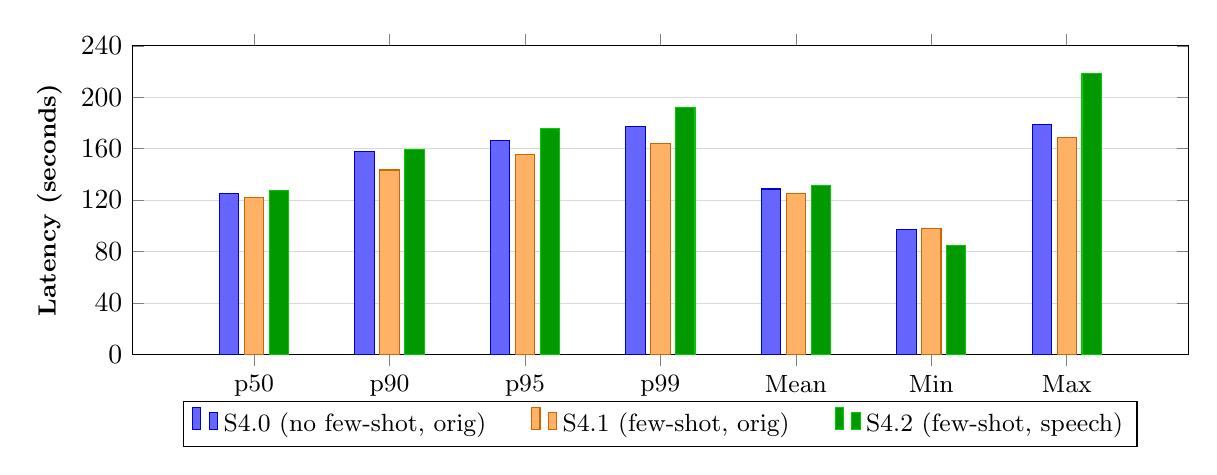
\begin{tikzpicture}
  \begin{axis}[
    width=15cm,
    height=5.5cm,
    ybar,
    bar width=7pt,
    ylabel={Latency (seconds)},
    ylabel style={font=\small\bfseries},
    xlabel={Statistics},
    xlabel style={font=\small\bfseries},
    symbolic x coords={p50, p90, p95, p99, Mean, Min, Max},
    xtick=data,
    xticklabel style={font=\small},
    ymin=0,
    ymax=240,
    ytick={0, 40, 80, 120, 160, 200, 240},
    ymajorgrids=true,
    grid style={line width=0.3pt, draw=gray!30},
    legend style={
      at={(0.5,-0.15)},
      anchor=north,
      legend columns=3,
      font=\small,
      /tikz/every even column/.append style={column sep=0.5cm}
    },
    enlarge x limits=0.15,
  ]
  
  % S4.0 (no few-shot, orig) - Blue
  \addplot[fill=blue!60, draw=blue!80!black] coordinates {
    (p50, 125.14)
    (p90, 157.96)
    (p95, 166.02)
    (p99, 177.27)
    (Mean, 128.64)
    (Min, 97.08)
    (Max, 179.00)
  };
  \addlegendentry{S4.0 (no few-shot, orig)}
  
  % S4.1 (few-shot, orig) - Orange
  \addplot[fill=orange!60, draw=orange!80!black] coordinates {
    (p50, 121.81)
    (p90, 143.39)
    (p95, 155.16)
    (p99, 164.08)
    (Mean, 124.98)
    (Min, 98.10)
    (Max, 168.81)
  };
  \addlegendentry{S4.1 (few-shot, orig)}
  
  % S4.2 (few-shot, speech) - Green
  \addplot[fill=green!60!black, draw=green!80!black] coordinates {
    (p50, 127.23)
    (p90, 159.02)
    (p95, 175.50)
    (p99, 192.16)
    (Mean, 131.15)
    (Min, 84.42)
    (Max, 218.22)
  };
  \addlegendentry{S4.2 (few-shot, speech)}
  
  \end{axis}
\end{tikzpicture}
\caption{Latency statistics for S4 variants (seconds). The per-field multi-LLM strategy shows the highest computational cost, with median latencies near 2 minutes and p99 values above 3 minutes. Few-shot prompting (S4.1) slightly lowers extreme latencies relative to S4.0, while the speech-style variant (S4.2) adds more variance. Overall, S4 highlights the trade-off between the robustness of per-field consensus and the considerable runtime required for multiple LLM calls.}
\label{fig:s4-latency-bar}
\end{figure}

Figure~\ref{fig:s4-latency-bar} makes clear that S4 is the slowest strategy family. All three variants have median latencies in the 122–127\,s range per document and heavy upper tails, with p99 values between roughly $164$\,s and $192$\,s. This behaviour is expected because S4 runs multiple models for each individual slot rather than once per document. Few-shot prompting slightly reduces median and mean latency when moving from S4.0 to S4.1, but the differences are small compared to the overall cost of per-field ensemble processing. S4.2 is marginally slower than S4.1 on average and exhibits the heaviest tail (Max above $218$\,s), reflecting additional variability in convergence on speech-style inputs. In comparison to S3.1, which also uses multi-LLM consensus but at the document level, S4 sacrifices throughput for more aggressive slot-level filling; this makes it less attractive for high-volume or time-sensitive deployments unless very high recall on nonempty fields is the primary objective.

\subsection*{Cost Analysis (S4: Multi-LLM Per-Field Consensus)}

\textbf{Assumptions.} For each of the $F{=}9$ fields, two parallel extractions are run—\textit{GPT-5} and \textit{Gemini~2.5~Pro}—with per-field averages $i_f{=}1{,}500$ input tokens and $o_f{=}50$ output tokens. A single arbiter/verification step per record runs on \textit{GPT-5-mini} with $V_{\text{in}}{=}1{,}000$ and $V_{\text{out}}{=}100$. If audio is used, Whisper transcription for $D$ minutes is added once per record.

\textbf{Prices.} GPT-5: input \$1.25/M, output \$10.00/M. Gemini~2.5~Pro: input \$1.25/M, output \$10.00/M. GPT-5-mini: input \$0.25/M, output \$2.00/M. Whisper: \$0.006/min.

\textbf{Formula.}
\[
\text{Cost}_{\text{S4}} =
\sum_{f=1}^{F}\!\Big[
\underbrace{\tfrac{i_f}{10^6}p_{\text{in}}^{(5)} + \tfrac{o_f}{10^6}p_{\text{out}}^{(5)}}_{\text{GPT-5 per field}}
+
\underbrace{\tfrac{i_f}{10^6}p_{\text{in}}^{(\text{Gemini})} + \tfrac{o_f}{10^6}p_{\text{out}}^{(\text{Gemini})}}_{\text{Gemini per field}}
\Big]
+\underbrace{\tfrac{V_{\text{in}}}{10^6}p_{\text{in}}^{(\text{mini})}+\tfrac{V_{\text{out}}}{10^6}p_{\text{out}}^{(\text{mini})}}_{\text{single arbiter}}
+0.006\cdot D
\]

\textbf{Per-record (no audio).}
\[
\begin{aligned}
\text{Per field (GPT-5): } & \tfrac{1500}{10^6}\!\cdot\!1.25 + \tfrac{50}{10^6}\!\cdot\!10.00 = \$0.002375 \\
\text{Per field (Gemini): } & \tfrac{1500}{10^6}\!\cdot\!1.25 + \tfrac{50}{10^6}\!\cdot\!10.00 = \$0.002375 \\
\text{Both models per field: } & \$0.00475 \\
\text{Across }F{=}9\text{ fields: } & 9 \times 0.00475 = \$0.04275 \\
\text{Arbiter (mini, once): } & \tfrac{1000}{10^6}\!\cdot\!0.25 + \tfrac{100}{10^6}\!\cdot\!2.00 = \$0.00045 \\
\textbf{Total: } & \mathbf{\$0.04320}\ (\approx 4.32\text{¢/doc})
\end{aligned}
\]

\textbf{With audio (Whisper).} Adding Whisper introduces a linear term $0.006\cdot D$. For $D{=}1$\,min, the total cost becomes $\$0.04320 + 0.006 = \mathbf{\$0.04920}$ (approximately $4.92$\,¢ per document). At these settings, S4 costs about $6\times$ as much as S1 (\$0.04320 vs.\ \$0.00720 per document, no audio) and roughly $2\times$ as much as S2 (\$0.04320 vs.\ \$0.02183), with the main driver being the per-field dual-model passes; the single-record arbiter remains a relatively minor component of the overall cost.

\subsection*{Consistency (Formatting \& Style)}

Figure~\ref{fig:s4-consistency} shows that S4 maintains reasonably high structural and stylistic consistency despite its aggressive fill behaviour. All variants achieve $\mathrm{FPR}_{\text{overall}}$ above $0.87$, and few-shot prompting again helps: S4.1 and S4.2 reach $0.94$, closing most of the gap to the best-performing strategies in this regard. Style-aware consistency $\mathrm{SC}_{\text{macro}}$ increases from $0.6599$ in S4.0 to $0.6881$ in S4.1, with a small drop to $0.6815$ for S4.2 on speech-style input. This suggests that the combination of per-slot prompting and consensus does not destabilise output formatting, even though the model ensemble is more willing to produce content in marginal cases.

Taken together, the S4 results characterise multi-LLM per-field consensus as an aggressive, recall-oriented strategy. It achieves high NES and strong performance on genuinely nonempty slots, particularly for context-sensitive fields such as \texttt{incidentLocation}, but this comes at the cost of elevated hallucination rates, negative EAI, and substantially higher latency and monetary cost. Compared to full-document consensus (S3.1), S4.1 offers higher NES (0.624 vs.\ 0.521) but lower OBS (0.579 vs.\ 0.641) because it overfills when gold is empty. In scenarios where maximising content recall on nonempty slots is critical and throughput is less of a concern, S4.1 is a compelling option—especially if combined with downstream post-filters. For more balanced deployments that must trade off accuracy, calibration, latency, and cost, S3.1 provides a more favourable operating point than S4’s per-field ensemble.```

\begin{figure}[H]
\centering
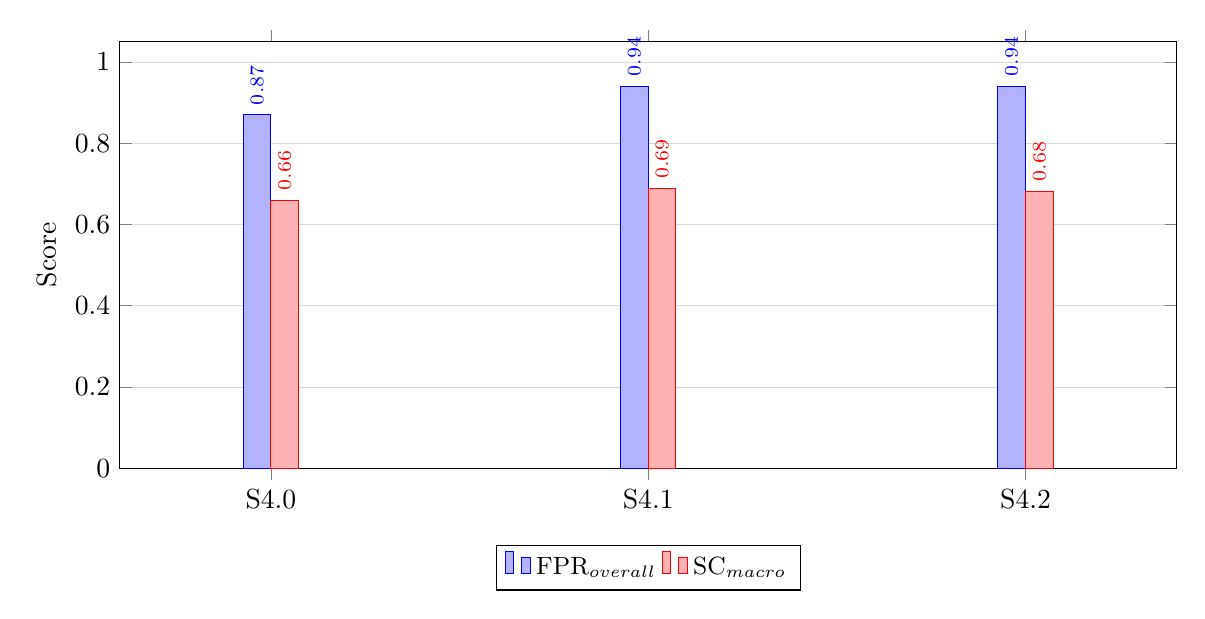
\begin{tikzpicture}
  \begin{axis}[
    width=15cm,
    height=7cm,
    ybar=0pt,
    bar width=10pt,
    ymin=0, ymax=1.05,
    ylabel={Score},
    symbolic x coords={S4.0,S4.1,S4.2},
    xtick=data,
    ymajorgrids=true,
    grid style={line width=0.3pt, draw=gray!30},
    legend style={at={(0.5,-0.18)}, anchor=north, legend columns=2, font=\small},
    enlarge x limits=0.20,
    nodes near coords,
    nodes near coords style={
        font=\scriptsize,
        rotate=90,     % vertical text
        anchor=west,
    }
  ]
    % FPR_overall
    \addplot coordinates {(S4.0,0.870) (S4.1,0.940) (S4.2,0.940)};
    \addlegendentry{$\mathrm{FPR}_{\text{overall}}$}

    % SC_macro
    \addplot coordinates {(S4.0,0.6599) (S4.1,0.6881) (S4.2,0.6815)};
    \addlegendentry{$\mathrm{SC}_{\text{macro}}$}
  \end{axis}
\end{tikzpicture}
\caption{Consistency (S4 variants): schema formatting vs.\ input-aware style.}
\label{fig:s4-consistency}
\end{figure}


\section{Comparative Analysis of Strategies}
\label{sec:eval-comparative}

This section compares the four Invox strategies (S1, S2, S3, S4) on the same dataset to identify their relative strengths and trade-offs. All results use few-shot prompting on the original MUC-4 test set (N=100).

\subsection*{Accuracy Comparison}

Figure~\ref{fig:strategy-comparison-bar} shows the main performance metrics. S1.1 reaches the highest OBS (0.644) and SF1 (0.642), with low hallucination (HR = 0.180). S4.1 has the highest NES (0.624), meaning it performs best when gold values exist, but its HR is much higher (0.476), indicating it often fills empty fields incorrectly. S2.1 and S3.1 fall between these extremes. The Empty Advantage Index (EAI) shows how much each strategy benefits from correctly leaving fields empty: S1.1 has EAI = 0.140, while S4.1 has negative EAI (-0.044), confirming it relies on filling rather than abstaining.
\begin{figure}[H]
\centering
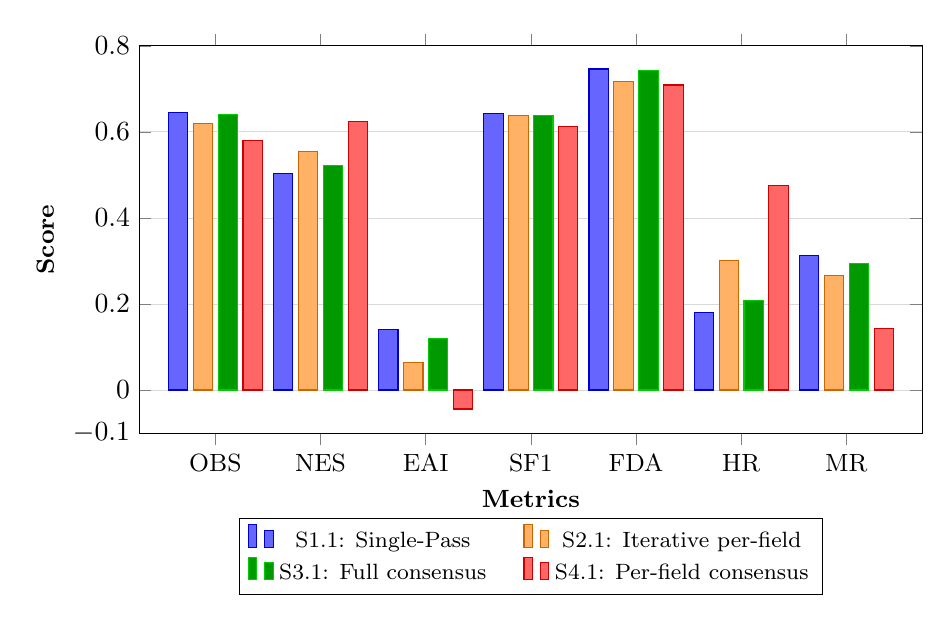
\begin{tikzpicture}
  \begin{axis}[
    width=0.95\textwidth,
    height=6.5cm,
    ybar,
    bar width=7pt,
    ylabel={Score},
    ylabel style={font=\small\bfseries},
    xlabel={Metrics},
    xlabel style={font=\small\bfseries},
    symbolic x coords={OBS, NES, EAI, SF1, FDA, HR, MR},
    xtick=data,
    xticklabel style={font=\small},
    ymin=-0.1,
    ymax=0.8,
    ytick={-0.1, 0, 0.2, 0.4, 0.6, 0.8},
    ymajorgrids=true,
    grid style={line width=0.3pt, draw=gray!30},
    legend style={
      at={(0.5,-0.22)},
      anchor=north,
      legend columns=2,
      font=\footnotesize,
      /tikz/every even column/.append style={column sep=0.4cm}
    },
    enlarge x limits=0.12,
  ]
  
  % S1.1: Single-Pass - Blue
  \addplot[fill=blue!60, draw=blue!80!black] coordinates {
    (OBS, 0.644) (NES, 0.504) (EAI, 0.140) (SF1, 0.642)
    (FDA, 0.746) (HR, 0.180) (MR, 0.313)
  };
  \addlegendentry{S1.1: Single-Pass}
  
  % S2.1: Iterative per-field - Orange
  \addplot[fill=orange!60, draw=orange!80!black] coordinates {
    (OBS, 0.619) (NES, 0.555) (EAI, 0.064) (SF1, 0.639)
    (FDA, 0.718) (HR, 0.301) (MR, 0.267)
  };
  \addlegendentry{S2.1: Iterative per-field}
  
  % S3.1: Full consensus - Green
  \addplot[fill=green!60!black, draw=green!80!black] coordinates {
    (OBS, 0.641) (NES, 0.521) (EAI, 0.120) (SF1, 0.638)
    (FDA, 0.743) (HR, 0.208) (MR, 0.295)
  };
  \addlegendentry{S3.1: Full consensus}
  
  % S4.1: Per-field consensus - Red
  \addplot[fill=red!60, draw=red!80!black] coordinates {
    (OBS, 0.579) (NES, 0.624) (EAI, -0.044) (SF1, 0.613)
    (FDA, 0.709) (HR, 0.476) (MR, 0.144)
  };
  \addlegendentry{S4.1: Per-field consensus}
  
  \end{axis}
\end{tikzpicture}
\caption{Performance comparison across four strategies (few-shot, orig MUC-4).}
\label{fig:strategy-comparison-bar}
\end{figure}


\subsection*{Cost Comparison}

Figure~\ref{fig:cost-trend-audio} shows how cost increases with audio duration. All strategies add \$0.006 per minute for Whisper transcription. The base LLM cost varies: S1.1 costs 0.72\textcent, S3.1 costs 1.40\textcent, S2.1 costs 2.18\textcent, and S4.1 costs 4.32\textcent per document (without audio). At 1 minute of audio, S4.1 is 3.7$\times$ more expensive than S1.1.
\begin{figure}[H]
\centering
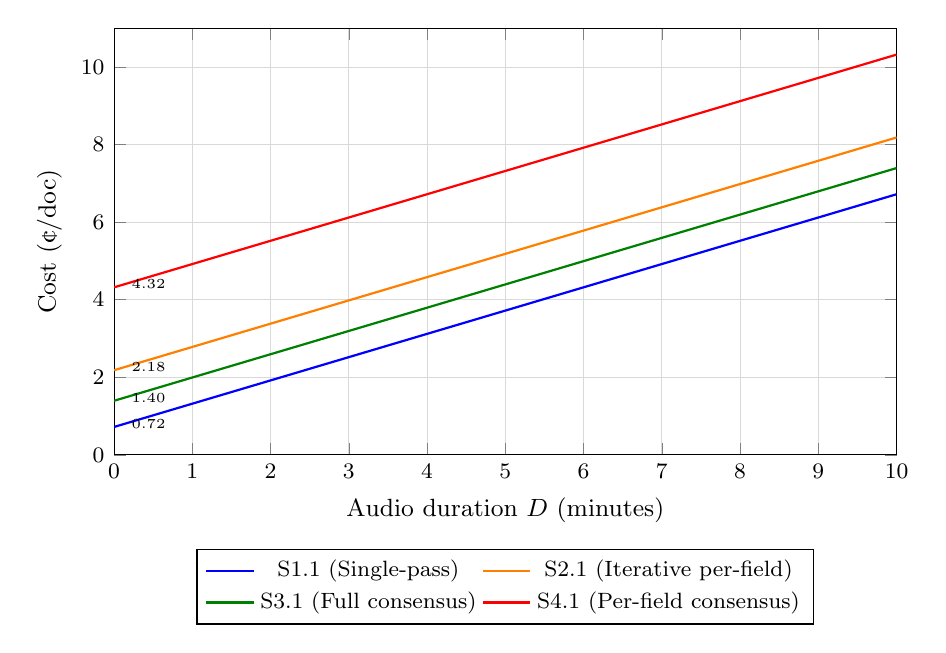
\begin{tikzpicture}
  \begin{axis}[
    width=0.95\textwidth, 
    height=7cm,
    xlabel={Audio duration $D$ (minutes)},
    ylabel={Cost (\textcent/doc)},
    xlabel style={font=\small},
    ylabel style={font=\small},
    xmin=0, xmax=10,
    ymin=0, ymax=11,
    grid=both,
    grid style={line width=0.3pt, draw=gray!30},
    legend style={at={(0.5,-0.22)}, anchor=north, legend columns=2, font=\footnotesize},
    domain=0:10,
    samples=2,
    tick label style={font=\footnotesize},
  ]

  % Removed "mark=*" from all lines
  \addplot+[thick, no markers, color=blue]  {0.72  + 0.60*x};
  \addlegendentry{S1.1 (Single-pass)}

  \addplot+[thick, no markers, color=orange] {2.183 + 0.60*x};
  \addlegendentry{S2.1 (Iterative per-field)}

  \addplot+[thick, no markers, color=green!50!black] {1.395 + 0.60*x};
  \addlegendentry{S3.1 (Full consensus)}

  \addplot+[thick, no markers, color=red] {4.32  + 0.60*x};
  \addlegendentry{S4.1 (Per-field consensus)}

  % Baseline labels
  \node[anchor=west, font=\tiny] at (axis cs:0.1,0.80) {0.72};
  \node[anchor=west, font=\tiny] at (axis cs:0.1,2.26) {2.18};
  \node[anchor=west, font=\tiny] at (axis cs:0.1,1.47) {1.40};
  \node[anchor=west, font=\tiny] at (axis cs:0.1,4.40) {4.32};

  \end{axis}
\end{tikzpicture}
\caption{Cost vs.\ audio duration: $\text{cost}(D)=\text{base}+0.60D$ (\textcent/doc).}
\label{fig:cost-trend-audio}
\end{figure}


\subsection*{Latency Comparison}


\begin{figure}[H]
\centering
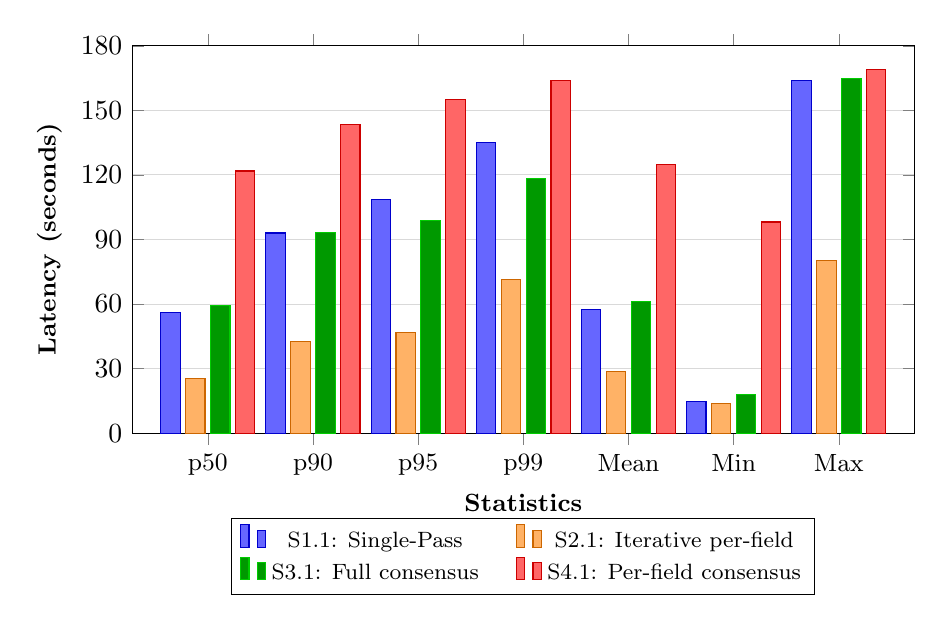
\begin{tikzpicture}
  \begin{axis}[
    width=0.95\textwidth,
    height=6.5cm,
    ybar,
    bar width=7pt,
    ylabel={Latency (seconds)},
    ylabel style={font=\small\bfseries},
    xlabel={Statistics},
    xlabel style={font=\small\bfseries},
    symbolic x coords={p50, p90, p95, p99, Mean, Min, Max},
    xtick=data,
    xticklabel style={font=\small},
    ymin=0,
    ymax=180,
    ytick={0, 30, 60, 90, 120, 150, 180},
    ymajorgrids=true,
    grid style={line width=0.3pt, draw=gray!30},
    legend style={
      at={(0.5,-0.22)},
      anchor=north,
      legend columns=2,
      font=\footnotesize,
      /tikz/every even column/.append style={column sep=0.4cm}
    },
    enlarge x limits=0.12,
  ]
  
  % S1.1: Single-Pass - Blue
  \addplot[fill=blue!60, draw=blue!80!black] coordinates {
    (p50, 55.91) (p90, 93.01) (p95, 108.40) (p99, 134.93)
    (Mean, 57.34) (Min, 14.54) (Max, 163.79)
  };
  \addlegendentry{S1.1: Single-Pass}
  
  % S2.1: Iterative per-field - Orange
  \addplot[fill=orange!60, draw=orange!80!black] coordinates {
    (p50, 25.35) (p90, 42.48) (p95, 46.68) (p99, 71.52)
    (Mean, 28.58) (Min, 13.60) (Max, 80.28)
  };
  \addlegendentry{S2.1: Iterative per-field}
  
  % S3.1: Full consensus - Green
  \addplot[fill=green!60!black, draw=green!80!black] coordinates {
    (p50, 59.39) (p90, 93.15) (p95, 98.77) (p99, 118.28)
    (Mean, 61.09) (Min, 18.13) (Max, 164.96)
  };
  \addlegendentry{S3.1: Full consensus}
  
  % S4.1: Per-field consensus - Red
  \addplot[fill=red!60, draw=red!80!black] coordinates {
    (p50, 121.81) (p90, 143.39) (p95, 155.16) (p99, 164.08)
    (Mean, 124.98) (Min, 98.10) (Max, 168.81)
  };
  \addlegendentry{S4.1: Per-field consensus}
  
  \end{axis}
\end{tikzpicture}
\caption{Latency distribution across strategies (seconds).}
\label{fig:latency-comparison-bar}
\end{figure}



\subsection*{Consistency Comparison}

Figure~\ref{fig:consistency-cross-strategy} compares how well each strategy follows the schema format (FPR$_{\text{overall}}$) and maintains consistent writing style (SC$_{\text{macro}}$). The baseline S5 (LangExtract) has perfect format compliance (1.000) because it uses strict validation rules. Among Invox strategies, S1.1 has the highest format score (0.960). For style consistency, S1.1 and S3.1 both reach 0.724, slightly higher than S2.1 (0.683) and S4.1 (0.688).

\begin{figure}[H]
\centering
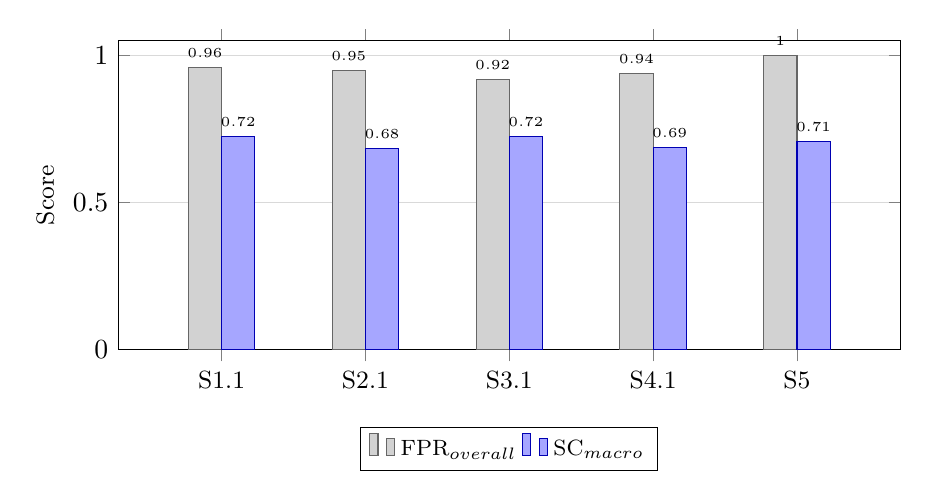
\begin{tikzpicture}
  \begin{axis}[
    width=0.95\textwidth,
    height=5.5cm,
    ybar=0pt,
    bar width=12pt,
    ymin=0, ymax=1.05,
    ylabel={Score},
    ylabel style={font=\small},
    symbolic x coords={S1.1,S2.1,S3.1,S4.1,S5},
    xtick=data,
    xticklabel style={font=\small},
    ymajorgrids=true,
    grid style={line width=0.3pt, draw=gray!30},
    legend style={at={(0.5,-0.25)}, anchor=north, legend columns=2, font=\footnotesize},
    enlarge x limits=0.18,
    nodes near coords,
    nodes near coords style={font=\tiny},
    nodes near coords align={vertical},
  ]
    \addplot[fill=gray!35, draw=black!60] coordinates {
      (S1.1,0.960) (S2.1,0.950) (S3.1,0.920) (S4.1,0.940) (S5,1.000)
    };
    \addlegendentry{$\mathrm{FPR}_{\text{overall}}$}

    \addplot[fill=blue!35, draw=blue!70!black] coordinates {
      (S1.1,0.724) (S2.1,0.683) (S3.1,0.724) (S4.1,0.688) (S5,0.709)
    };
    \addlegendentry{$\mathrm{SC}_{\text{macro}}$}
  \end{axis}
\end{tikzpicture}
\caption{Format compliance and style consistency across strategies.}
\label{fig:consistency-cross-strategy}
\end{figure}


\subsection*{Observed Trade-offs}

The four strategies show clear patterns:

\textbf{S1.1 (Single-LLM Full-Input)} achieves the best overall scores (OBS = 0.644), balancing accuracy, speed (median 55.91s), cost (0.72\textcent), and lowest hallucination (0.180).

\textbf{S2.1 (Single-LLM One-Field)} is fastest (median 25.35s) through parallel processing. Accuracy is slightly lower (OBS = 0.619) with higher hallucination (0.301), but improves location fields.

\textbf{S3.1 (Multi-LLM Full-Input)} runs two models, reducing hallucination (HR = 0.208) and improving NES (0.521 vs.\ 0.504). Speed and cost fall between S1.1 and S2.1.

\textbf{S4.1 (Multi-LLM One-Field)} runs two models per field, achieving highest NES (0.624) and lowest missing rate (0.144), but highest hallucination (0.476). It is slowest (median 121.81s) and most expensive (4.32\textcent).

The main trade-off is filling correctly when values exist (NES, MR) versus abstaining when absent (HR, EAI). S1.1 and S3.1 balance both. S2.1 prioritizes speed. S4.1 prioritizes recall over precision.

